\documentclass{article}
\usepackage[utf8]{inputenc}
\usepackage{amsmath}
\usepackage{amssymb}
\usepackage{graphicx}

\begin{document}

\section*{Non linear electric circuit}
In this problem we deal with a very simple non-linear circuit element, a diode. The current $I$ through a diode to which a voltage $U$ is applied can be modelled by the relationship
\begin{equation*}
    I = \alpha\left(e^{\beta\frac{U}{U_{T}}}-1\right)
\end{equation*}
with suitable paramteters $\alpha, \beta > 0$ and the thermal voltage $U_{T}$. We consider the following circuit

\begin{figure}[!hbt]
    \centering
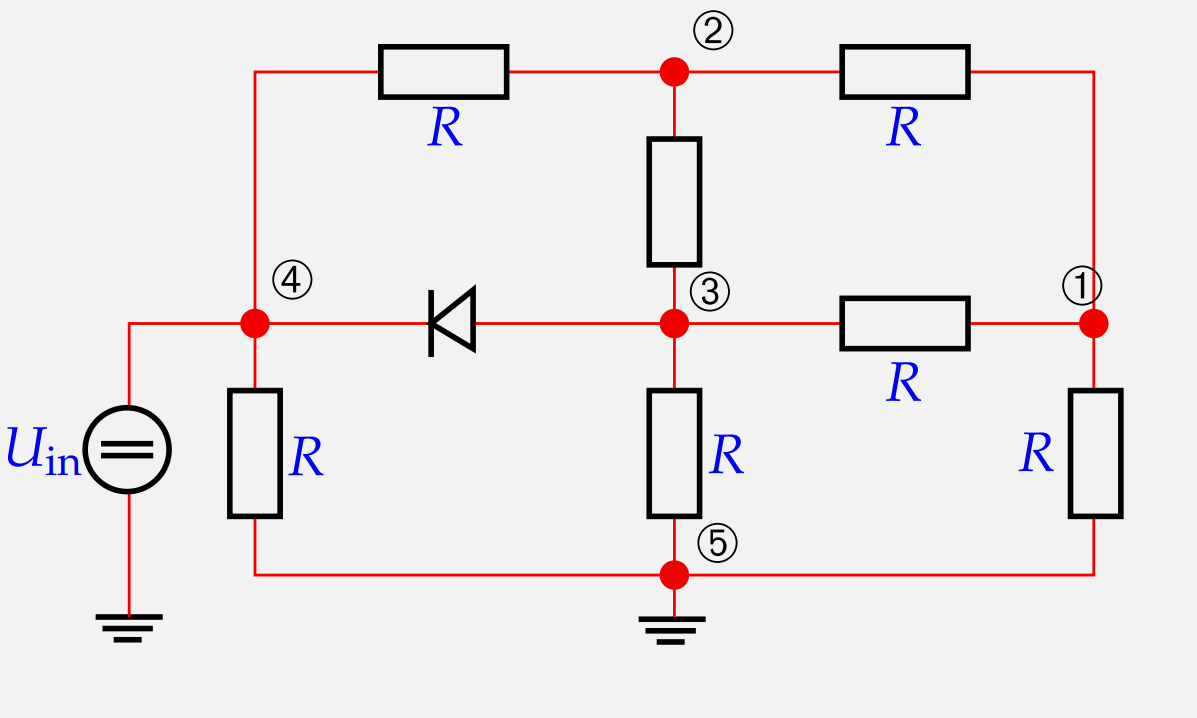
\includegraphics[width=0.7\linewidth]{NodalAnalysis8-7.png}
\end{figure}

We assume that all resistors have non-dimensional resistance $R=1$. The circuit is driven by imposing a voltage $U_{\text{in}}$ through an ideal voltage source.
\subsection*{8-7.a}
We are tasked with studying the relevant part of the lecture document again to refresh our non-existent knowledge about nodal analysis of electric circuits. The red dots depicted above are \textbf{Nodes}, which are junction of wires. Each node has a number which is used to denote the current between two nodes, the current $I_{kj}$ denotes the current flowing from node $k$ to the node $j$. We then have $I_{kj}=-I_{jk}$. The most fundamental relationship is the \textbf{Kirchhoff current law} that demande that the sum od node current vanishes
\begin{equation*}
    \forall \, k \in \left\{1, \dots, n\right\}\::\: \sum_{j=1}^{n}I_{kj} = 0
\end{equation*}
The unknowns of the model are the \textbf{nodal} potentials $U_{k}$, $k=1, \dots, n$. We also have the important relation for the Ohmic resistor
\begin{equation*}
    I = \frac{U}{R}
\end{equation*}
here we have $R=1$, hence this equation simplifies (in this special case) to $U = I$. From this we can derive that $I_{kj} = R^{-1}\left(U_{k} - U_{j}\right)$.
\subsection*{8-7.b}
We are tasked with finding a non-linear system of equations $\mathbf{F}\left(\mathbf{u}\right) = \mathbf{0}$ for the potentials in nodes $1$, $2$ and $3$, where the voltages in nodes $4$ and $5$ are known given input voltage $U_{in}$ and ground voltage (the upside down pyramid in the figure) $0$. We apply the Kirchoff current law for each node while using $I_{kj} = R^{-1}\left(U_{k} - U_{j}\right) = U_{k} - U_{j}$ (only in this example, because $R=1$) for each of the resistors.
\begin{align*}
    0&=\left(U_{2} - U_{1}\right) + \left(U_{3} - U_{1}\right) + \left(U_{5} - U_{1}\right) \\
    0&=\left(U_{1} - U_{2}\right) + \left(U_{3} - U_{2}\right) + \left(U_{4} - U_{2}\right)  \\ 0&=
    \left(U_{1} - U_{3}\right) + \left(U_{2} - U_{3}\right) + \left(U_{5} - U_{3}\right) - \alpha\left(e^{\beta\left(\frac{U_{3}-U_{\text{in}}}{U_{T}}\right)}-1\right)
\end{align*}
Because $U_{5}$ is connected to ground and $U_{4}$ is connected to $U_{\text{in}}$ we have
\begin{equation*}
    U_{5} = 0 \quad U_{4} = U_{\text{in}}
\end{equation*}
This means that our system simplifies to 
\begin{align*}
    0&=\left(U_{2} - U_{1}\right) + \left(U_{3} - U_{1}\right) + \left(0 - U_{1}\right) \\
    0&=\left(U_{1} - U_{2}\right) + \left(U_{3} - U_{2}\right) + \left(U_{\text{in}} - U_{2}\right) \\
   0&= \left(U_{1} - U_{3}\right) + \left(U_{2} - U_{3}\right) + \left(0- U_{3}\right) - \alpha\left(e^{\beta\left(\frac{U_{3}-U_{\text{in}}}{U_{T}}\right)}-1\right)
\end{align*}
Which furthermore can be simplified to 
\begin{align*}
    0 &= U_{2} + U_{3} - 3U_{1}\\
    0&= U_{1} + U_{3} + U_{\text{in}} -3U_{2} \\
    0 &= U_{1} + U_{2} - \alpha\left(e^{\beta\left(\frac{U_{3}-U_{\text{in}}}{U_{T}}\right)}-1\right) -3U_{3}
\end{align*}
We then use
\begin{equation*}
 \alpha\left(e^{\beta\left(\frac{U_{3}-U_{\text{in}}}{U_{T}}\right)}-1\right) =  \alpha e^{\beta\left(\frac{U_{3}-U_{\text{in}}}{U_{T}}\right)} - \alpha =   \alpha e^{\left(\frac{\beta}{U_{T}}U_{3} - \frac{\beta}{U_{T}}U_{\text{in}}\right)} - \alpha = \alpha e^{\frac{\beta}{U_{T}}U_{3}} \cdot e^{-\frac{\beta}{U_{T}}U_{\text{in}}} - \alpha
\end{equation*}
Which gives us the following nonlinear system of equations (We multiplied the system by $-1$ to )
\begin{equation*}
    \begin{bmatrix}
    3U_{1} - U_{2} - U_{3} \\
    3U_{2} - U_{1} - U_{3} - U_{\text{in}} \\
    3U_{3} - U_{1} - U_{2}  + \alpha e^{\frac{\beta}{U_{T}}U_{3}} \cdot e^{-\frac{\beta}{U_{T}}U_{\text{in}}} - \alpha
    \end{bmatrix} = 
    \begin{bmatrix}
        0 \\ 0 \\ 0
    \end{bmatrix} \text{ with } \begin{bmatrix}
        U_{1} \\
        U_{2} \\
        U_{3}
        \end{bmatrix}
\end{equation*}
I was trying for a second to transform this into a system in the form we know as $\mathbf{A}\mathbf{x} = \mathbf{b}$, but since this is a \textbf{non-linear} system of equations that is not possible.

\subsection*{8-7.c}
We are tasked with implementing a function that computes the output voltages at node $1$ for a sorted vector of input voltages $U_{\text{in}}$ at node $4$ and for a thermal voltage $U_{T} = 0.5$, we are also given the parameters $\alpha$ and $\beta$. We are told to use Newton's method to solve $\mathbf{F}\left(\mathbf{x}\right) = \mathbf{0}$ with a relative tolerance of $\tau = 10^{-6}$. The iteration method of the multi-dimensional Newton method is
\begin{equation*}
    \mathbf{x}^{\left(k+1\right)} := \mathbf{x}^{\left(k\right)} - \mathrm{D}F\left(\mathbf{x}^{\left(k\right)}\right)^{-1}F\left(\mathbf{x}^{\left(k\right)}\right)
\end{equation*}
here the unknown is $\mathbf{u} = \mathbf{x}$, hence we will use the following notation
\begin{equation*}
    \mathbf{u}^{\left(k+1\right)} := \mathbf{u}^{\left(k\right)} - \mathrm{D}F\left(\mathbf{u}^{\left(k\right)}\right)^{-1}F\left(\mathbf{u}^{\left(k\right)}\right)
\end{equation*}
The Jacobian is given by 
\begin{align*}
    \mathrm{D}F\left(\mathbf{u}^{\left(k\right)}\right) = 
    \begin{bmatrix}
        \frac{\partial F_{1}}{\partial U_{1}} &  \frac{\partial F_{1}}{\partial U_{2}} & \frac{\partial F_{1}}{\partial U_{3}}  \\[1mm]
        \frac{\partial F_{2}}{\partial U_{1}} &  \frac{\partial F_{2}}{\partial U_{2}} & \frac{\partial F_{2}}{\partial U_{3}}  \\[1mm]
        \frac{\partial F_{3}}{\partial U_{1}} &  \frac{\partial F_{3}}{\partial U_{2}} & \frac{\partial F_{3}}{\partial U_{3}}  
    \end{bmatrix} &= \begin{bmatrix}
        3 & -1 & -1 \\
        -1 & 3 & -1 \\
        -1 & -1 & 3 + \alpha e^{-\frac{\beta}{U_{T}}U_{in}}\cdot e^{\frac{\beta}{U_{T}}U_{3}}\cdot \frac{\beta}{U_{T}}
    \end{bmatrix} \\
    &= \begin{bmatrix}
        3 & -1 & -1 \\
        -1 & 3 & -1 \\
        -1 & -1 & 3 + \frac{\alpha\beta}{U_{T}} \cdot e^{\beta\frac{U_{3}-U_{\text{in}}}{U_{T}}}
    \end{bmatrix}
\end{align*}
We then have a look at the following code segment from the lecture document (8.5.1.8)

\begin{figure}[!hbt]
    \centering
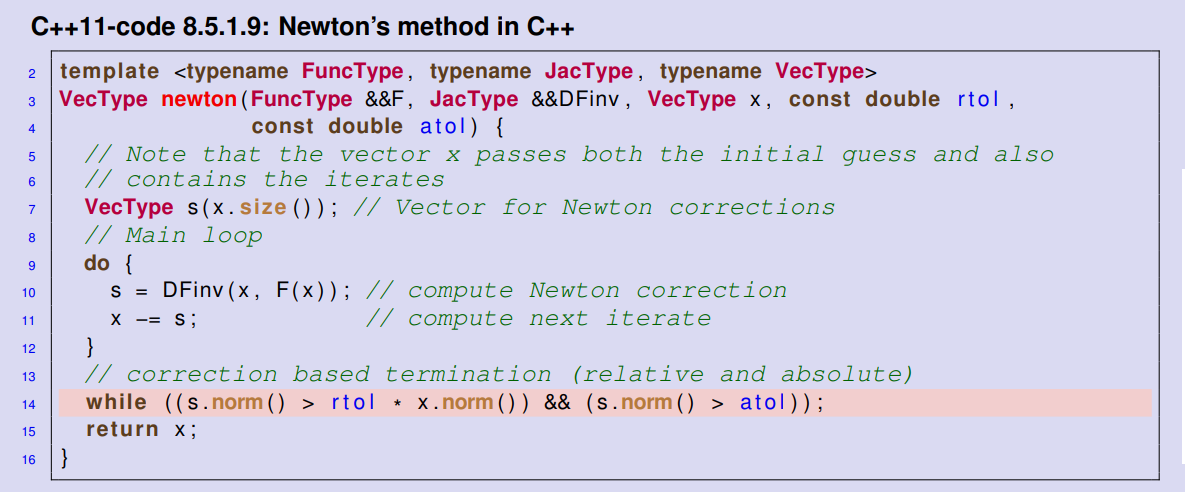
\includegraphics[width=1.0\linewidth]{CodeNewtonMethod.png}
\end{figure}

\noindent Here we only want to use a relative tolerance, hence we leave the \verb|atol| part out. We could also add it by choosing something like $1E-8$ as our absolute tolerance. We hence need to implement to functors for $F$ and $\mathrm{D}F$ first and then find a way to compute $\mathrm{D}F\left(\mathbf{u}^{\left(k\right)}\right)^{-1}$. As always we use the trick (this is a must know) denoting $\mathbf{x}$ as some placeholder variable, which does not refer to any prior symbols
\begin{equation*}
    \mathrm{D}F\left(\mathbf{u}^{\left(k\right)}\right)\mathbf{x} = F\left(\mathbf{u}^{\left(k\right)}\right) \Longleftrightarrow \mathbf{x} = \mathrm{D}F\left(\mathbf{u}^{\left(k\right)}\right)^{-1}F\left(\mathbf{u}^{\left(k\right)}\right)
\end{equation*}
This is an expression we can solve by using any of the decompositions and the use the \verb|solve()| method in Eigen. This produces the following code.

\begin{figure}[!hbt]
    \centering
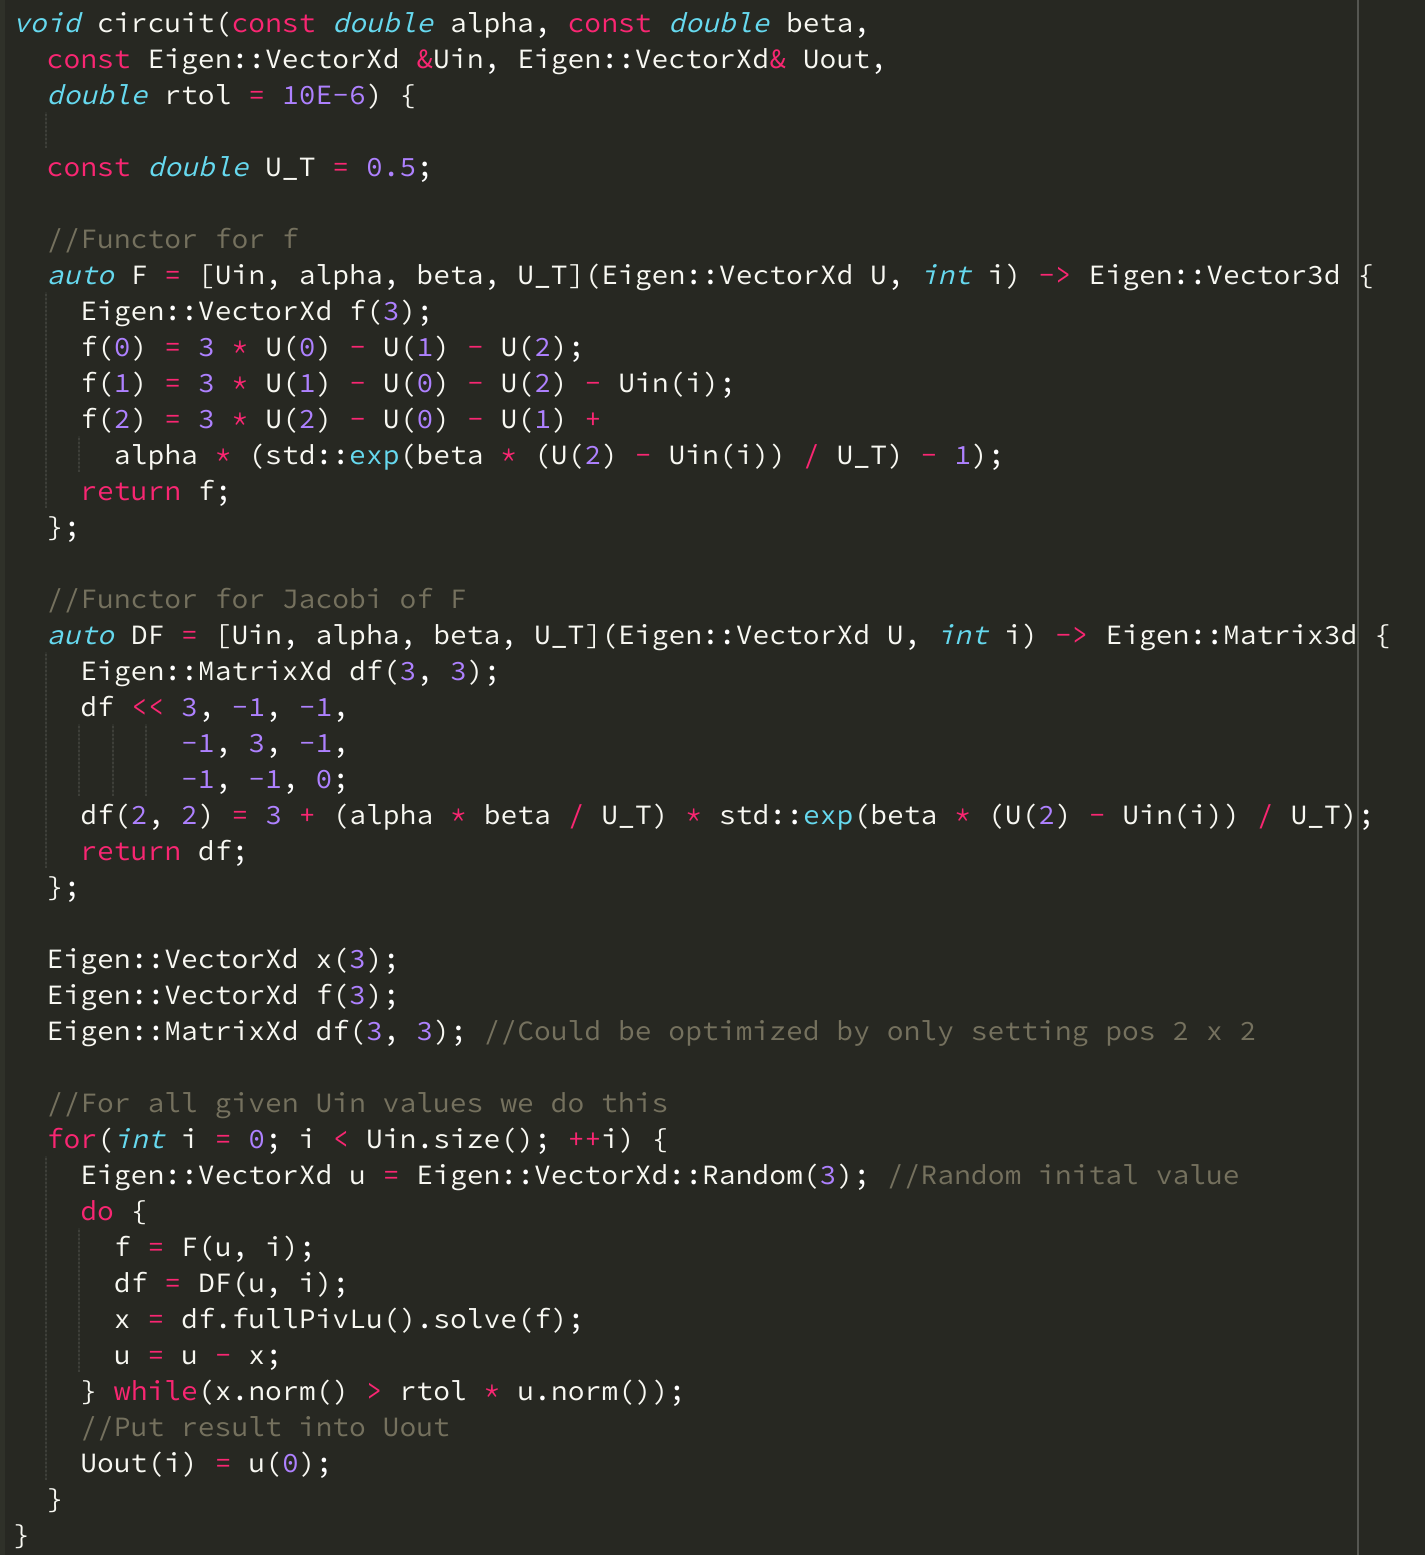
\includegraphics[width=1.0\linewidth]{8-7.c.png}
\end{figure}
\subsection*{8-7.d}
This exercise was skipped as it contributes very little to the understanding of the topics discussed in this exercise.
\end{document}
